\documentclass[a4paper, 12pt, titlepage]{article}

% Including needed packages
\usepackage[margin=2cm]{geometry}
\usepackage{amsmath}
\usepackage{amssymb}
\usepackage{amsthm}
\usepackage{graphicx}
\usepackage{subfig}
\usepackage{float}
\usepackage{pgf}
\usepackage{tikz}

\newcommand{\norm}[1]{\lVert#1\rVert}
\usetikzlibrary{automata,positioning}

\title
{{\em Machine learning 2}\\
Exercise sheet 9}
\author{FLEISCHMANN Kay, Matrnr: 352247\\
	ROHRMANN Till, Matrnr: 343756}
\date{\today}

\begin{document}

\maketitle

\section{Hidden Markov Models}
Let $A_{i,j}$ the transition matrix between hidden states $x_i$ and $x_j$. $B_{i,j}$ is the the probability, beeing in state $i$ to overserve $y_j$.
The following matrices $A$ and $B$ describe two hidden states and two possible observations.

\[
A= 
 \begin{pmatrix}
  0.1 & 0.9 \\
  0.5 & 0.5
 \end{pmatrix}
\]

\[
B=
 \begin{pmatrix}
  0.2 & 0.8 \\
  0.4 & 0.6
 \end{pmatrix}
\]

\subsection{a. Draw the graph of the model}
The Hidden-Markov-chain for $A$ and $B$ looks like the following4

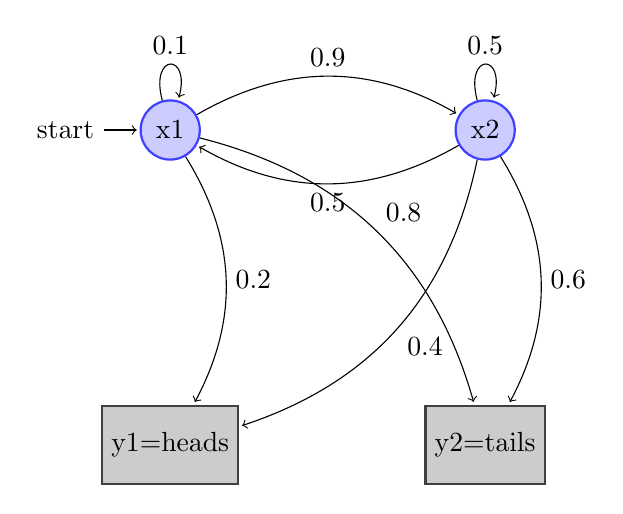
\begin{tikzpicture}[shorten >=1pt,node distance=2cm,on grid,auto] 
  \tikzstyle{state}=[circle,thick,draw=blue!75,fill=blue!20,minimum size=6mm]
  \tikzstyle{observation}=[rectangle,thick,draw=black!75,
  			  fill=black!20,minimum size=10mm]
  			  
  \node[state,initial] (x1)   {x1}; 
  \node[state] (x2) [right=4cm of x1] {x2};
  \node[observation] (y1) [below=4cm of x1] {y1=heads};
  \node[observation] (y2) [right=4cm of y1] {y2=tails};

  \path[->] (x1) edge [bend left] node {0.9} (x2);
  \path[->] (x2) edge [bend left] node {0.5} (x1);
  \path[->] (x1) edge [loop above] node {0.1} (x1);
  \path[->] (x2) edge [loop above] node {0.5} (x2);

  \path[->] (x1) edge [bend left] node {0.2} (y1);
  \path[->] (x1) edge [bend left] node {0.8} (y2);

  \path[->] (x2) edge [bend left] node {0.4} (y1);
  \path[->] (x2) edge [bend left] node {0.6} (y2);
\end{tikzpicture}
  
Because of $\pi = (1 | 0)$ all state-sequences start with the initial state $x_1$.
  
\subsection{b.}


\textit{We interpret the above as a model for an experiment with two hidden (unfair) coins and two visible coins. Describe such an experiment which can be modelled by the Markov model given above. Here, heads should correspond to the first indices in $A$, $B$, $\pi$, heads to the second.} \newline \newline
A man is standing behind an curtain and is throwing two unfair coins, just one each time. The guy in front of the curtain just get the observation wheter he sees heads or tails. 

\newpage
\subsection{c.}

Given the bayes rule:
\begin{equation}
   P(x|y_1=tails,y_2=tails) =  \frac{P(y_1=tails,y_2=tails|x)P(x)}{P(y_1=tails,y_2=tails)}
\end{equation}

Because of the statistical independence, we can write
\begin{equation}
  P(y_1=tail,y_2=tail|x_1,x_2) = \pi_1 \cdot P(y_1|x_1) \cdot P(x_1) \cdot P(y_2|x_2) \cdot P(x_2)
\end{equation}
In general, for the first two states which should produce the observation $(tails,tails)$ we can write

\begin{equation}
  P(y_1=tail,y_2=tail|x_1,x_2) = \pi_i \cdot P(y_1|x_i) \cdot P(x_i) \cdot P(y_2|x_i) \cdot P(x_i)
\end{equation}

All possible sequences with length $2$ are

\begin{tabular}{l*{3}{c}r}
              & State transitions & $P(x)$ & $P(y_1=tails,y_2=tails|x) $ \\
\hline
1 &  $x_1 \rightarrow x_1$ & $P(x_1,x_1)= 1\cdot0.1=0.1$ & $ 1\cdot0.4\cdot0.1\cdot0.4=0,016 $\\
2 &  $x_1 \rightarrow x_2$ & $P(x_1,x_2)= 1\cdot0.9=0.9$ & $ 1\cdot0.4\cdot0.9\cdot0.6=0,216 $ \\
3 &  $x_2 \rightarrow x_1$ & $P(x_2,x_1)= 0\cdot0.5=0$ & $ 0 $ \\
4 &  $x_2 \rightarrow x_2$ & $P(x_2,x_2)= 0\cdot0.5=0$ & $ 0 $
 \end{tabular}

\begin{align}
  P(y_1,y_2) &= \sum_{x} P(y_1,y_2|x) P(x)  \\
	     &= \sum_{x} P(y_1=tails,y_2=tails|x) P(x) \\
	     &= 0.016 \cdot 0.1 + 0.216 \cdot 0.9 \\
	     &= 0.196
\end{align}

The result for $P(x|y_1=tails,y_2=tails)$ follows as

\begin{tabular}{l*{2}{c}r}
              & State-sequence &  $P(x|y_1=tails,y_2=tails)$ & \\
\hline
& & & \\
1 & $x=x_1,x_1$ & $\frac{0.016 \cdot 0.1}{0.196} = 0.008163265$ \\
& & & \\
2 & $x=x_1,x_2$ & $\frac{0.216 \cdot 0.09}{0.196} =0.099183673$ \\
& & & \\
3 & $x=x_2,x_1$ & $\frac{0\cdot 0.45}{0.196} = 0$ \\
& & & \\
4 & $x=x_2,x_2$ & $\frac{0 \cdot 0.45}{0.196} = 0 $ 
 \end{tabular}





\end{document}